\chapter{Конструкторская часть}

В данном разделе будут представлены схемы реализаций алгоритмов сортировки, среди которых блинный, быстрый и сортировка бусинами.

\section{Разработка алгоритма блинной сортировки}
На рисунке \ref{img:pancake} представлена схема реализации алгоритма блинной сортировки. На рисунках \ref{img:ind_max} и \ref{img:flip} представлены схемы реализаций алгоритмов подпрограмм поиска индекса максимального элемента массива (рисунок \ref{img:ind_max}) и переворота массива (рисунок \ref{img:flip}), необходимых для реализации алгоритма блинной сортировки. Подпрограмма поиска индекса максимального элемента массива также используется в алгоритме сортировки бусинами.%, схема реализации которого приведена на рисунке \ref{img:bead}.

\begin{figure}[h!]
    \centering
    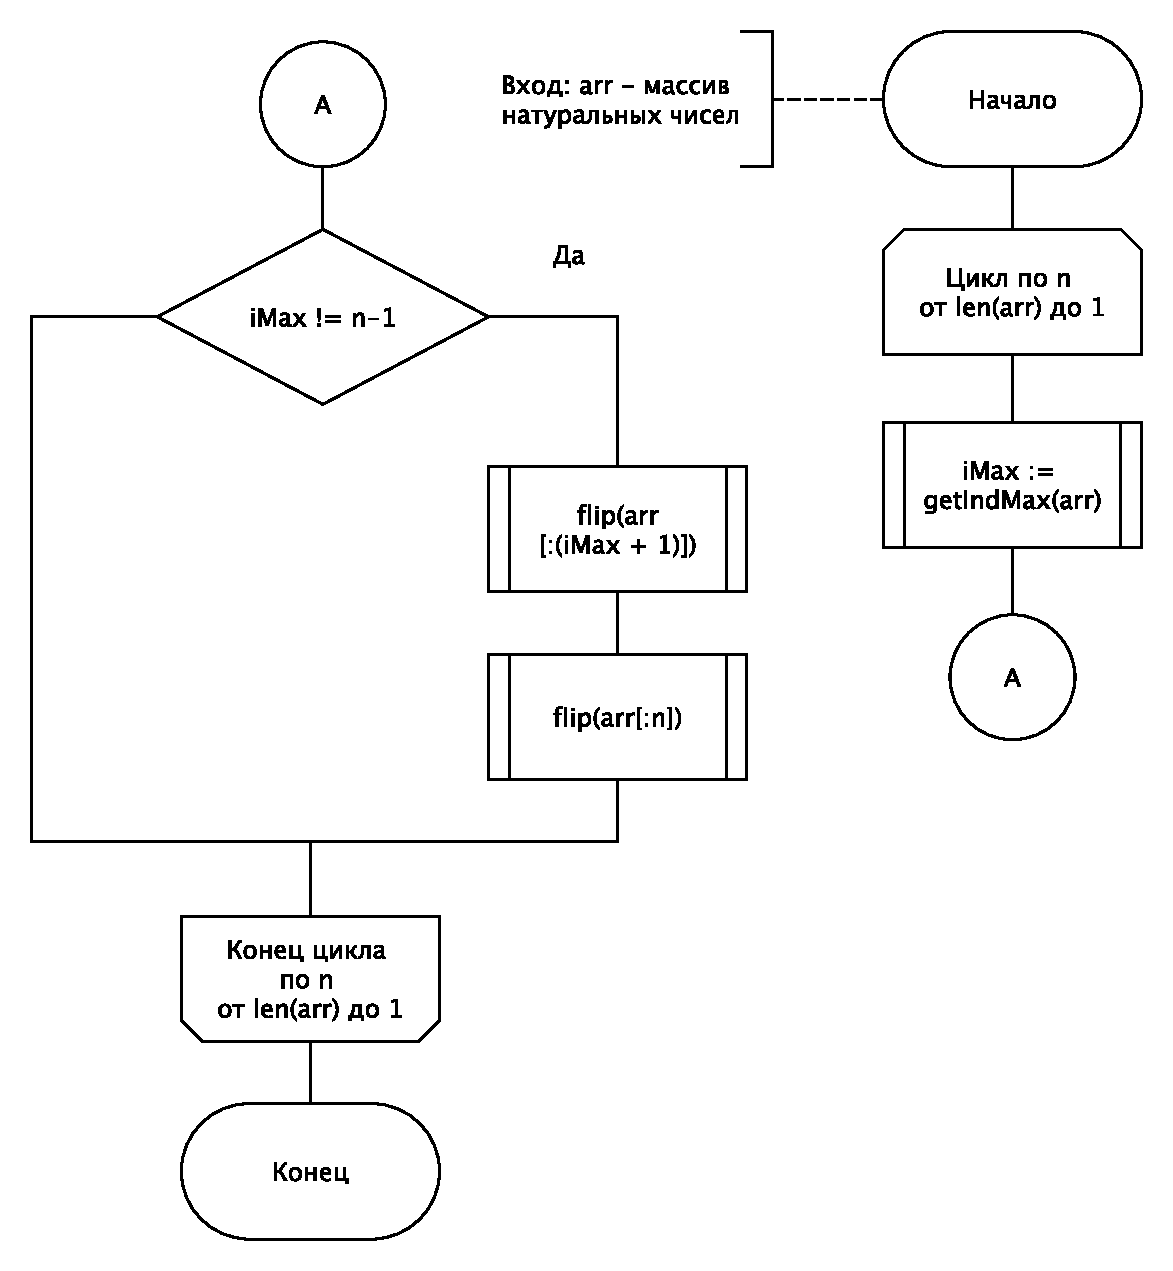
\includegraphics[width=0.65\linewidth]{pancake.pdf}
    \caption{Схема реализации алгоритма блинной сортировки}
    \label{img:pancake}
\end{figure}

\begin{figure}[h!]
    \centering
    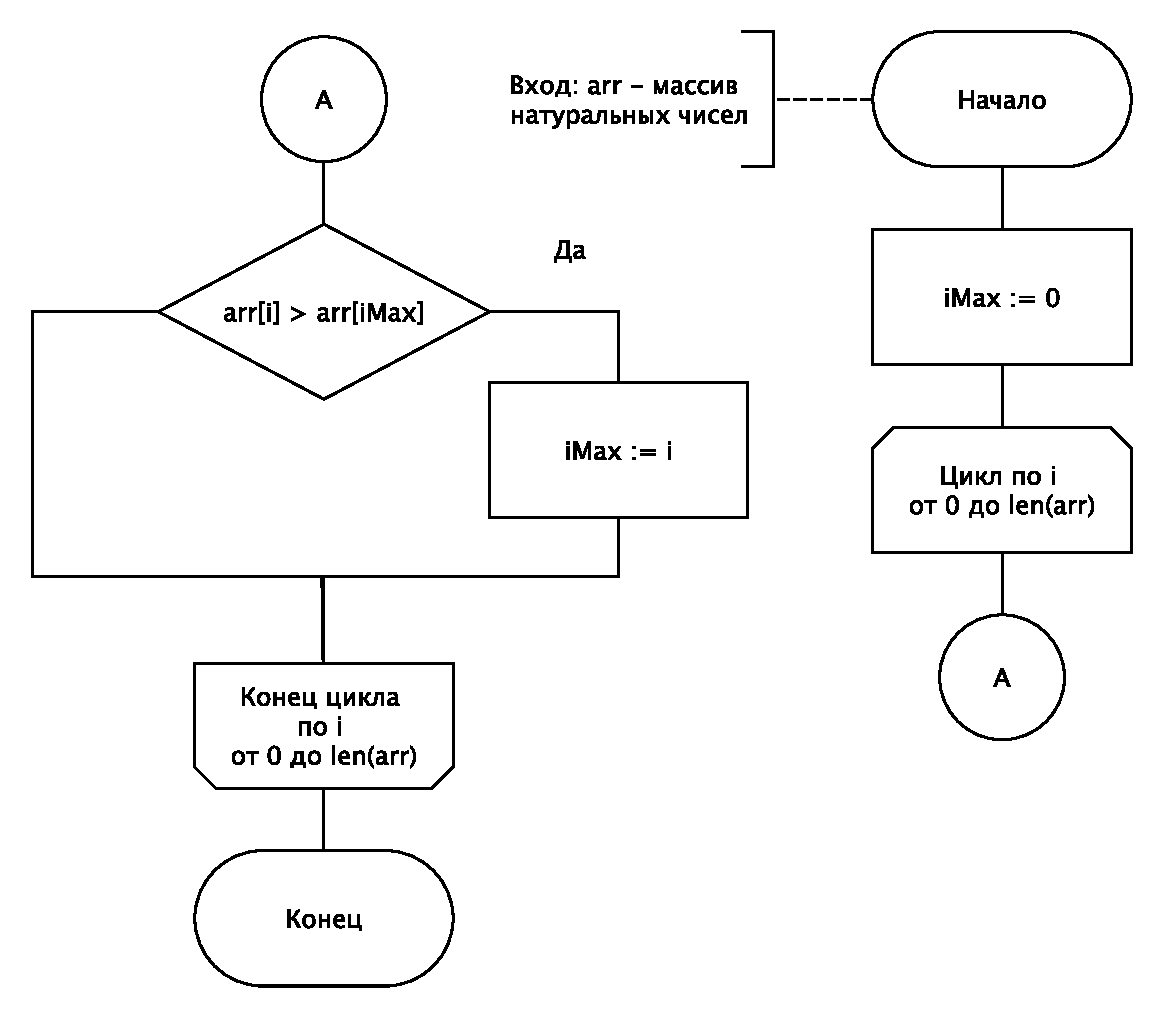
\includegraphics[width=0.6\linewidth]{ind_max.pdf}
    \caption{Схема реализации алгоритма поиска индекса максимального элемента массива}
    \label{img:ind_max}
\end{figure}

\begin{figure}[h!]
    \centering
    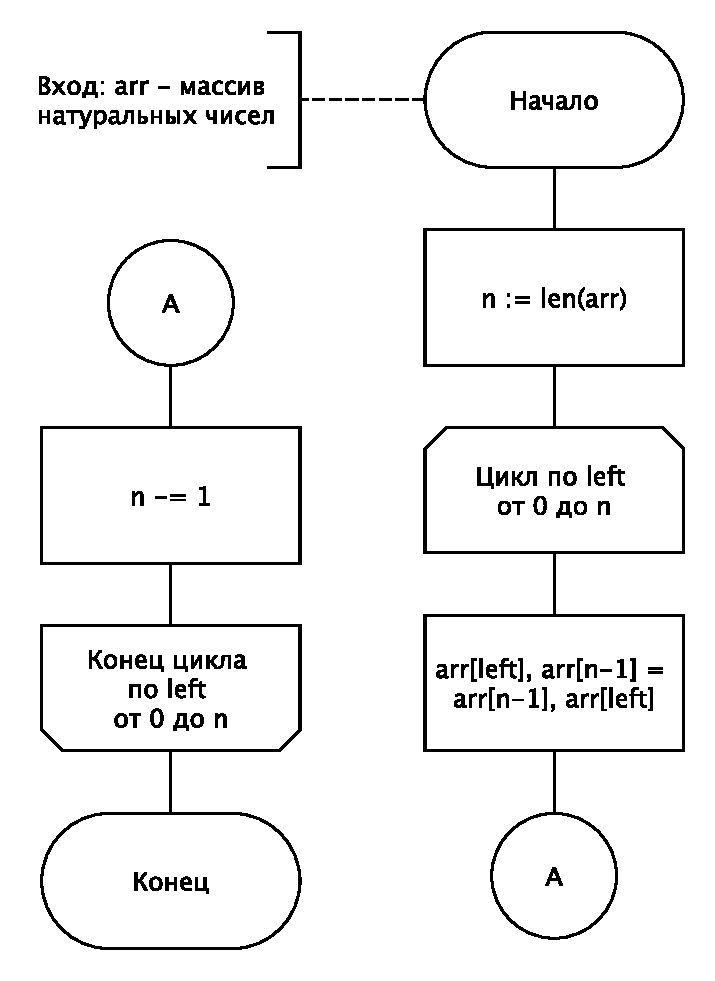
\includegraphics[width=0.45\linewidth]{flip.pdf}
    \caption{Схема реализации алгоритма переворота массива}
    \label{img:flip}
\end{figure}

\section{Разработка алгоритма быстрой сортировки}
На рисунке \ref{img:quick} представлена схема реализации алгоритма быстрой сортировки.

\begin{figure}[h!]
    \centering
    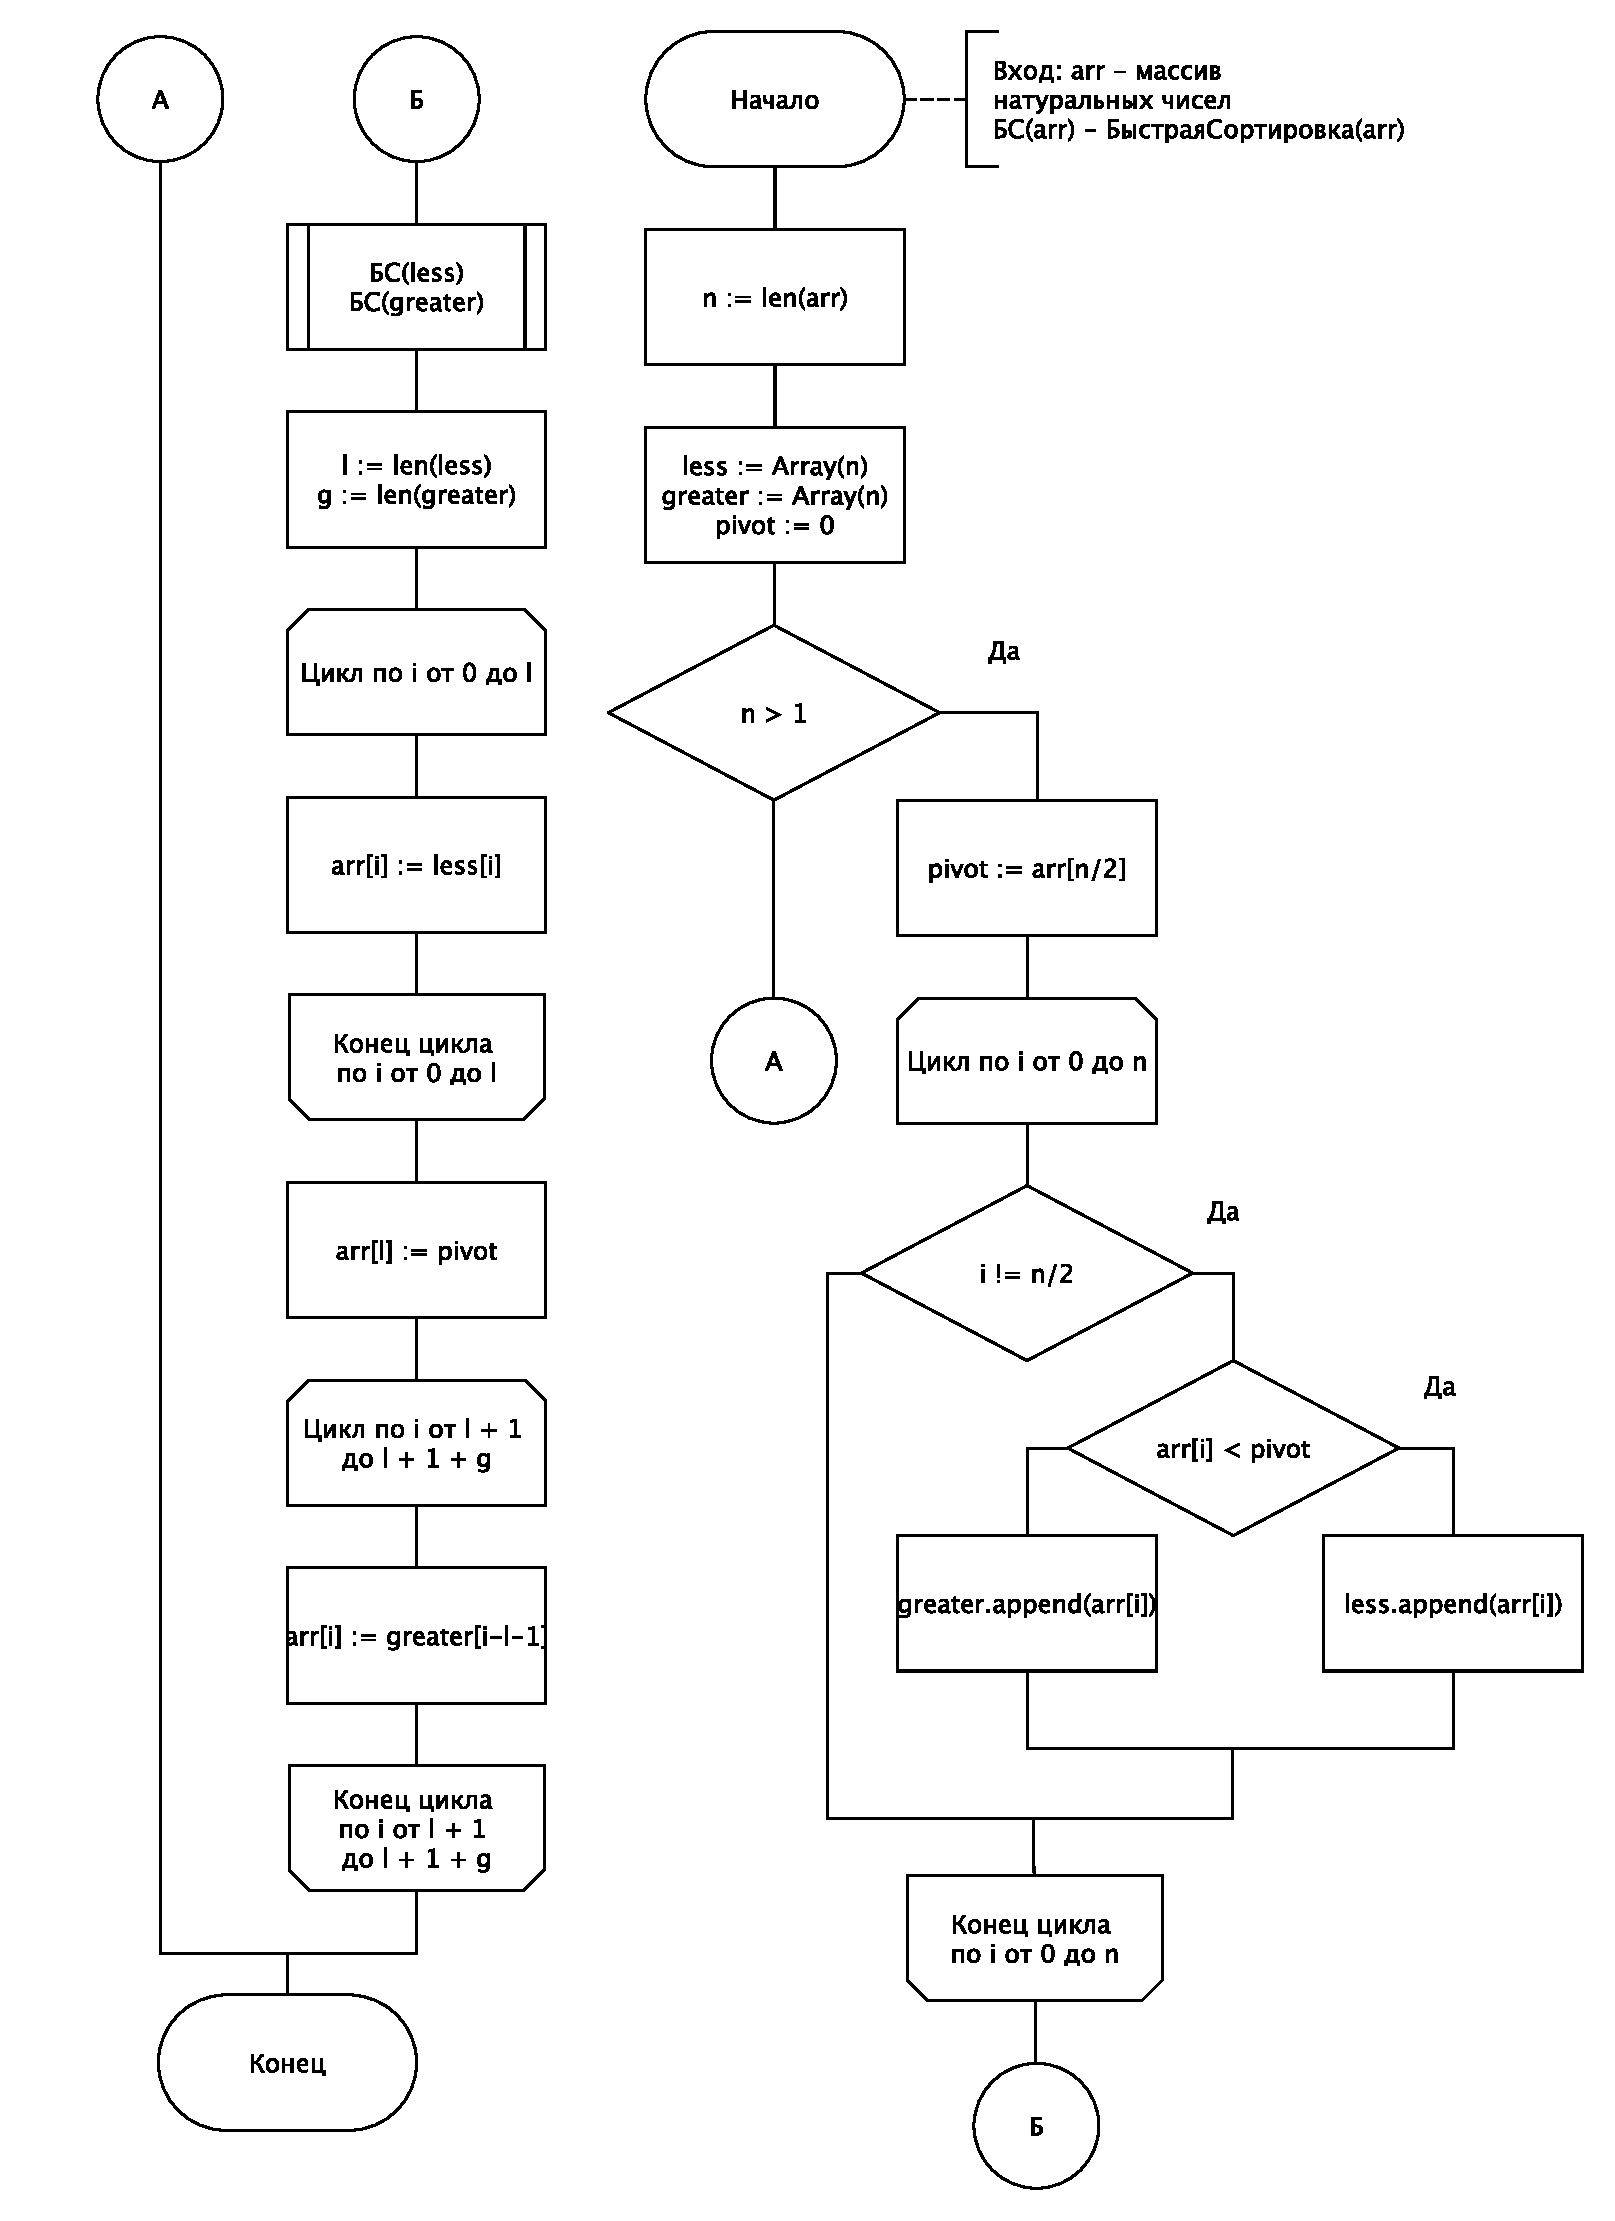
\includegraphics[width=0.82\linewidth]{quick.pdf}
    \caption{Схема реализации алгоритма быстрой сортировки}
    \label{img:quick}
\end{figure}

\section{Разработка алгоритма сортировки бусинами}
На рисунке \ref{img:bead} представлена схема реализации алгоритма cортировки бусинами. Алгоритм использует подпрограмму поиска индекса максимального элемента массива, схема которой приведена на рисунке \ref{img:ind_max}.

\begin{figure}[h!]
    \centering
    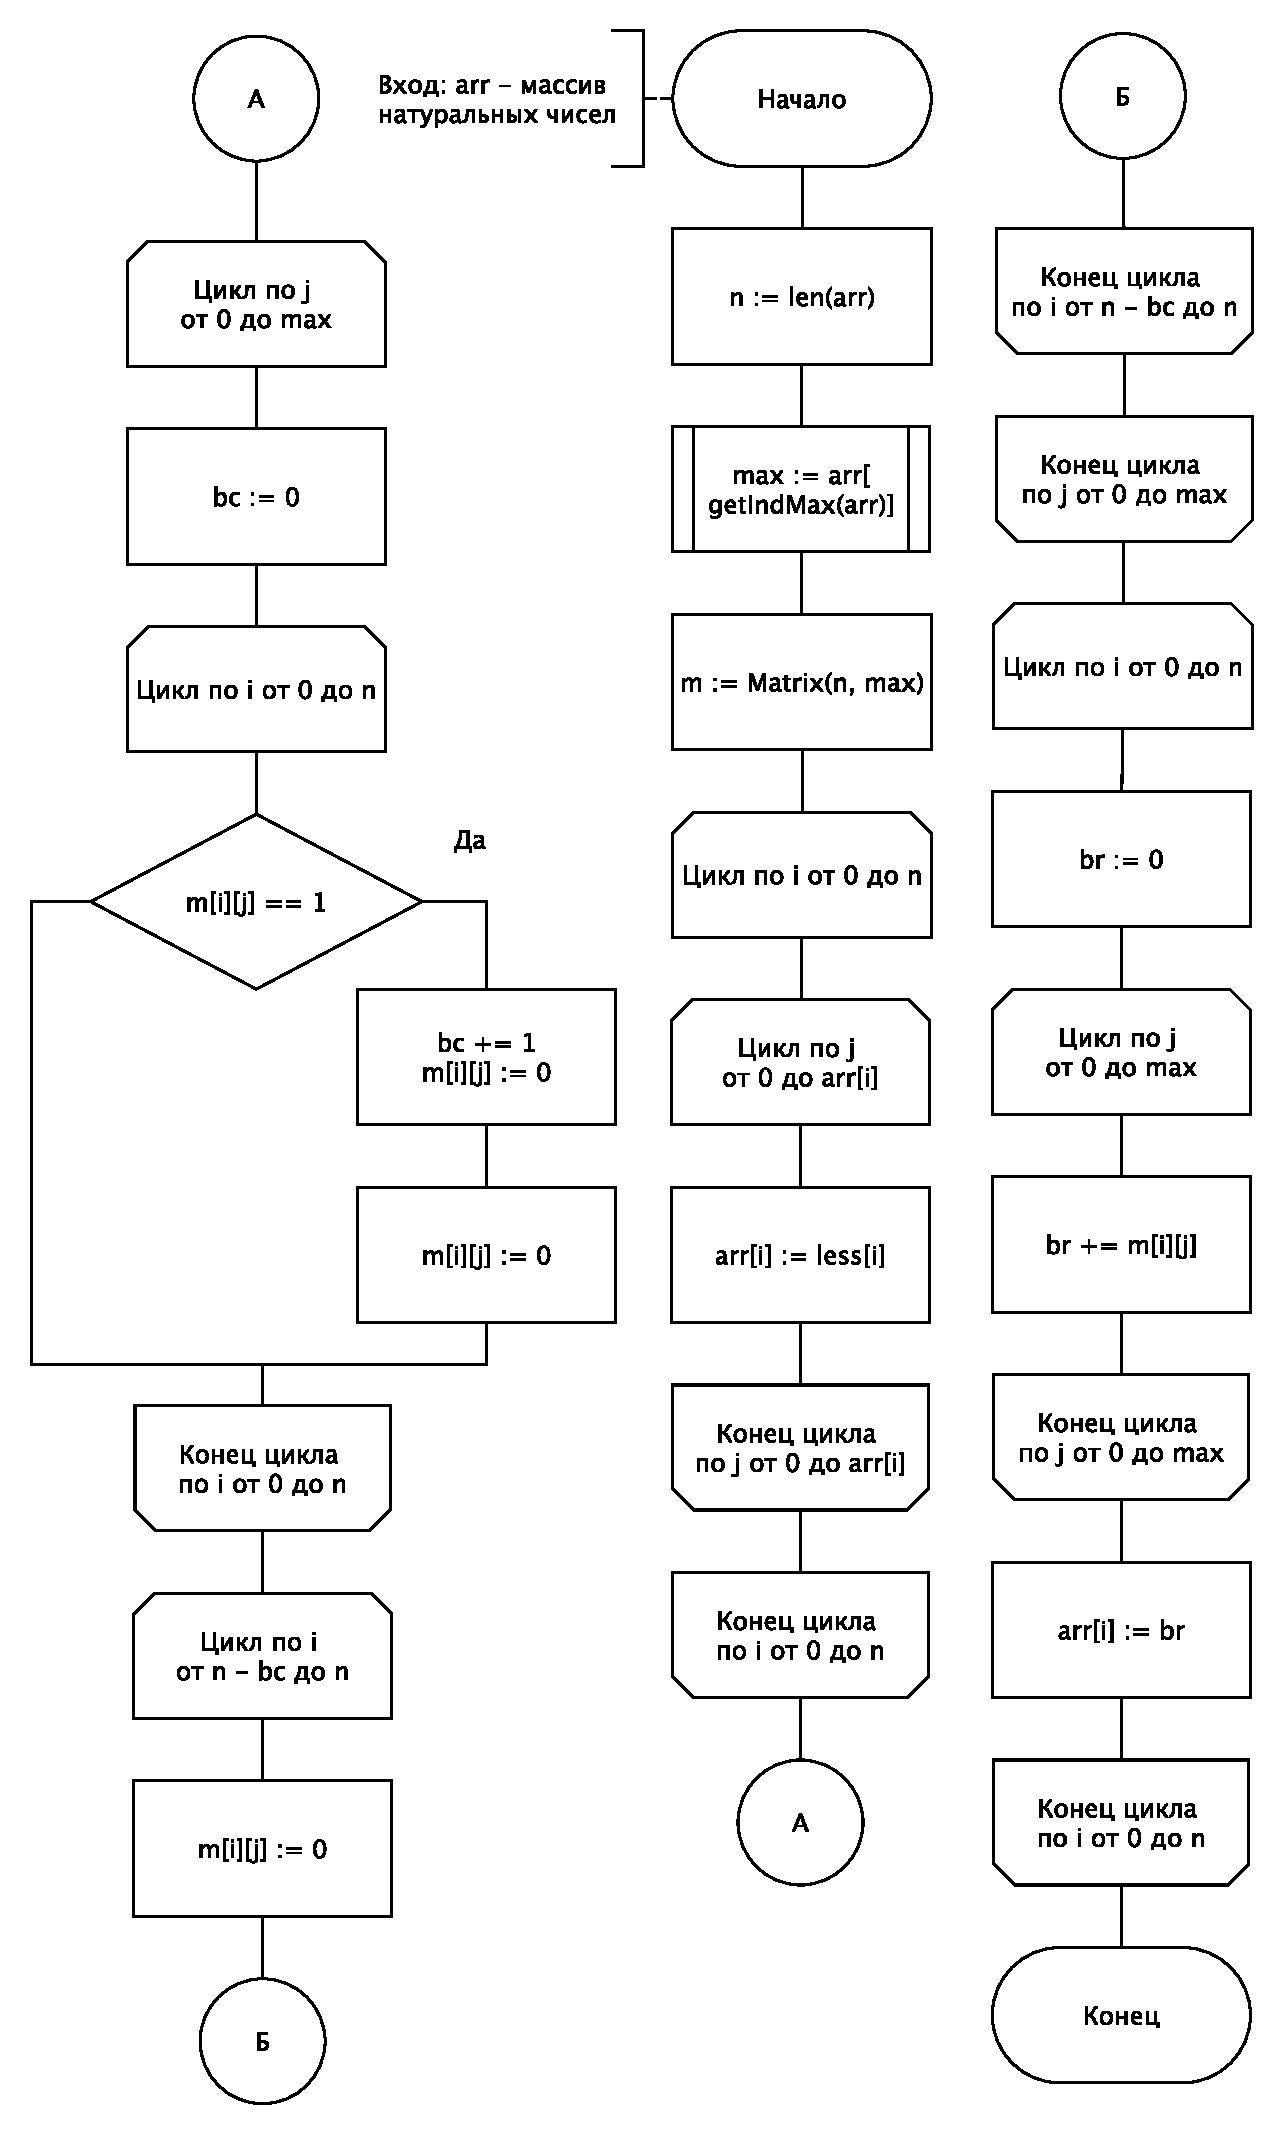
\includegraphics[width=0.66\linewidth]{bead.pdf}
    \caption{Схема реализации алгоритма cортировки бусинами}
    \label{img:bead}
\end{figure}

\newpage

\section{Модель вычислений}
Для вычисления трудоёмкости данных алгоритмов необходимо ввести модель вычислений.

Обозначим трудоёмкость \cite{web_item6} как $f_{a}$, где $a$~---~индекс, указывающий операцию, блок кода или оператор, для которого вычисляется трудоёмкость. \\

Определим трудоёмкость базовых операций как:
\begin{equation}
\begin{array}{rrrr}
	f_{+}=1 & \quad f_{-}=1 & \quad f_{+=}=1 & \quad f_{-=}=1 \\
	f_{:=}=1 & \quad f_{<<}=1 & \quad f_{>>}=1 & \quad f_{[]}=1 \\
	f_{++}=1 & \quad f_{--}=1 & \quad f_{>}=1 & \quad f_{<}=1 \\
	f_{>=}=1 & \quad f_{<=}=1 & \quad f_{!=}=1 & \quad f_{==}=1 \\
	f_{\cdot}=2 & \quad f_{/}=2 & \quad f_{\%}=2 & \quad \\
\end{array}
\end{equation}

Определим трудоёмкость вызова функции как $0$.

Определим трудоёмкость условия как

\begin{equation}
	f_{if} = f_{cc} + \begin{cases}
		\min(f_1, f_2),& \text{в лучшем случае}, \\
		\max(f_1, f_2),& \text{в худшем случае},
	\end{cases}
\end{equation}
где приняты следующие обозначения:
\begin{itemize}
	\item $f_{cc}$~---~трудоёмкость вычисления условия;
	\item $f_1$~---~трудоёмкость блока после $if$;
	\item $f_2$~---~трудоёмкость блока после $else$.
\end{itemize}

Определим трудоёмкость цикла как
\begin{equation}
	f_{loop} = f_{init} + f_{first_cmp} + n * (f_{body} + f_{inc} + f_{cmp}),
\end{equation}
где приняты следующие обозначения:
\begin{itemize}
	\item $f_{init}$~---~трудоёмкость инициализации;
	\item $f_{first_cmp}$~---~трудоёмкость первого сравнения;
	\item $f_{body}$~---~трудоёмкость тела цикла;
	\item $n$~---~количество итераций цикла;
	\item $f_{inc}$~---~трудоёмкость изменения индекса;
	\item $f_{cmp}$~---~трудоёмкость сравнения.
\end{itemize}

\section{Трудоёмкость алгоритмов сортировки}
Введём некоторые обозначения:
\begin{itemize}
	\item $N$~---~размерность массива;
	\item $f_{best}$~---~трудоёмкость алгоритма в лучшем случае;
	\item $f_{worst}$~---~трудоёмкость алгоритма в худшем случае.
\end{itemize}

\subsection{Трудоёмкость алгоритма блинной сортировки}
Рассчитаем трудоёмкость алгоритма блинной сортировки. Рассмотрим одну итерацию внешнего цикла $f_{n}$ для массива фиксированной длины $n$:
\begin{equation}
	f_{n} = 4 + f_{indMax} + 5 + \begin{cases}
		0,& \text{в лучшем случае (максимум в конце)}, \\
		f_{flip(n)} + f_{flip(n-1)},& \text{в худшем случае (иначе)}.
	\end{cases}
\end{equation}

При этом
\begin{equation}
	f_{indMax} = 3 + n \cdot  (3 + 2 + \begin{cases}
		0,& \text{в лучшем случае (максимум не сменился)}, \\
		1,& \text{в худшем случае (иначе)},
	\end{cases})
\end{equation}
то есть
\begin{equation}
	f_{indMax} = 3 + n \cdot  \begin{cases}
		5,& \text{в лучшем случае (максимум не сменился)}, \\
		6,& \text{в худшем случае (иначе)}.
	\end{cases}
\end{equation}

Также рассмотрим переворот элементов до максимума включая в ситуации худшего случая~---~когда максимумом является предпоследний элемент (приходится делать поворот для многих элементов):
\begin{equation}
	f_{flip(n-1)} = 3 + 11 \cdot  n
\end{equation}
и для переворота полного массива:
\begin{equation}
	f_{flip(n)} = 3 + 11 \cdot  n.
\end{equation}

Тогда для лучшего случая (в этом случае массив отсортирован по возрастанию, поэтому максимум будет обновляться на каждом шаге) будет получено соотношение
\begin{equation}
	f_{n} = 9 + 6 \cdot  n + 0 = 9 + 6 \cdot n,
\end{equation}
а для худшего (когда максимумами становятся предпоследние элементы относительно рассматриваемого массива, то есть большие и маленькие значения чередуются в массиве) будет получено соотношение
\begin{equation}
	f_{n} = 9 + n/2 \cdot  6 + n/2 \cdot  5 + 22 \cdot  n - 5 = 27.5 \cdot  n + 4.
\end{equation}

Таким образом
\begin{equation}
	f_{n} = \begin{cases}
		9 + 6 \cdot  n,& \text{в лучшем случае}, \\
		27.5 \cdot  n + 4,& \text{в худшем случае}.
	\end{cases}
\end{equation}

Для всего цикла будет получена последовательность
\begin{equation}
	f_{loop} = 2 + f_{2} + f_{3} + ... + f_{N},
\end{equation}
которую можно представить в виде арифметической прогрессии
\begin{equation}
	f_{loop} = 2 + \frac{f_{2} + f_{N}}{2} \cdot (N - 1).
\end{equation}

Итоговыми выражениями будут
\begin{equation}
\begin{cases}
	f = 3 \cdot N^2 + 10 \cdot N - 13,& \text{в лучшем случае}, \\
	f = \frac{27.5 \cdot N^2 + 35.5 \cdot N - 59}{2},& \text{в худшем случае}.
\end{cases}
\end{equation}

Можно сделать вывод, что асимптотика алгоритма блинной сортировки составляет $O(N^2)$ и в худшем, и в лучшем случаях.

\subsection{Трудоёмкость алгоритма быстрой сортировки}
Рассчитаем трудоёмкость алгоритма быстрой сортировки. Рассмотрим запуск функции на одной итерации и впоследствии умножим на глубину рекурсии. 

На одном запуске функции массив делится на части, каждая из которых обрабатывается рекурсивно данной функцией. Эти части в сумме образуют исходный массив, поэтому быстродействие одного рекурсивного погружения можно сравнить с быстродействием одной итерации на полном массиве, поэтому в данном расчёте используется значение $N$.

Тогда для одного вызова функции, кроме вызова для полного разбиения массива на части из одного элемента, который будет учтён позже
\begin{equation} \label{eqn:quick1}
	f = 8 + f_{loop} + 4 + f_{loopless} + f_{loopgreater}.
\end{equation}

При этом
\begin{equation}
	f_{loop} = 2 + (N - 1) \cdot (4 + f_{cond}) + 4,
\end{equation}
где последнее слагаемое соответствует обработке опорного элемента, а слагаемое в середине~---~остальным.

Обозначение $f_{cond}$ соответствует следующей формуле:
\begin{equation}
	f_{loop} = 2 + \begin{cases}
	1,& \text{если элемент меньше опорного}, \\
	1,& \text{если элемент больше или равен опорному}.
\end{cases}
\end{equation}

Также в формуле (\ref{eqn:quick1})
\begin{equation}
	f_{loopless} = 2 + 4 \cdot m,
\end{equation}
где 
\begin{equation}
	m = \begin{cases}
	\frac{N - 1}{2},& \text{в лучшем случае (равномерное разбиение)}, \\
	N - 1,& \text{в худшем случае (неравномерное разбиение)},
\end{cases}
\end{equation}
и
\begin{equation}
	f_{loopgreater} = 5 + 9 \cdot k,
\end{equation}
где 
\begin{equation}
	k = \begin{cases}
	\frac{N - 1}{2},& \text{в лучшем случае (равномерное разбиение)}, \\
	0,& \text{в худшем случае (неравномерное разбиение)}.
\end{cases}
\end{equation}

Тогда в промежуточной общей формуле
\begin{equation}
	f_{sub} = 18 + 7 \cdot N + 5 \cdot m + 9 \cdot k.
\end{equation}

В лучшем случае, то есть когда в массиве существует примерно равно количество элементов больше и элементов меньше опорного, глубина рекурсии составит $\log_2N$.

В худшем случае, когда опорный элемент является минимумом или максимумом последовательности, глубина рекурсии составит $N$.

Тогда после домножения результирующей формулы для одного погружения на соответствующие коэффициенты для двух случаев получается следующее соотношение:
\begin{equation}
	f = \begin{cases}
	f_{sub} \cdot \log_2N,& \text{в лучшем случае (равномерное разбиение)}, \\
	f_{sub} \cdot N,& \text{в худшем случае (неравномерное разбиение)}.
\end{cases}
\end{equation}

Осталось учесть итерации, на которых в функцию приходит массив из одного элемента:
\begin{equation}
	f = \begin{cases}
	f_{sub} \cdot (\log_2N - 1) + 5,& \text{в лучшем случае (равномерное разбиение)}, \\
	f_{sub} \cdot (N - 1) + 5,& \text{в худшем случае (неравномерное разбиение)}.
\end{cases}
\end{equation}

Можно сделать вывод, что асимптотика алгоритма быстрой сортировки составляет $O(N^2)$ в худшем случае, и $O(N \cdot \log_2N)$ в лучшем случае.

\newpage

\subsection{Трудоёмкость алгоритма сортировки бусинами (гравитационной)}
Рассчитаем трудоёмкость алгоритма сортировки бусинами.
\begin{equation} \label{eqn:bead1}
	f = 12 + f_{indMax} + N \cdot 3 + N \cdot a + c + (N \cdot (7 + m \cdot 5)).
\end{equation}

При этом
\begin{equation}
	f_{indMax} = 3 + N \cdot  (3 + 2 + \begin{cases}
		0,& \text{в лучшем случае (максимум не сменился)}, \\
		1,& \text{в худшем случае (иначе)},
	\end{cases}
\end{equation}

\begin{equation}
	a = 5 + m \cdot 6,
\end{equation}

\begin{equation}
	b = \begin{cases}
		4,& \text{при равенстве элемента матрицы единице}, \\
		0,& \text{иначе},
	\end{cases}
\end{equation}

\begin{equation}
	c = m \cdot (8 + N \cdot (5 + b) + N \cdot 5),
\end{equation}
а $m$~---~это максимальный элемент последовательности.

Так как худшим случаем для сортировки бусинами является ситуация, когда весь массив состоит из элементов с большими значениями, а лучший~---~из элементов с маленькими значениями, массивы при тестировании заполнялись одинаковыми элементами равными или размерности массива, или единице для двух случаев соответственно. Следовательно и значение $m$ всегда равнялось либо размерности массива, либо единице соответственно. От порядка значений в массиве быстродействие алгоритма или не меняется совсем, или меняется совсем незначительно. Поэтому для $f_{indMax}$ вариативная часть всегда будет равняться нулю, а $b$ всегда будет равняться 4.

После выполнения расчётов по (\ref{eqn:bead1}) получается следующее соотношение:
\begin{equation}
	f = 21 \cdot N + 25 \cdot m \cdot N + 8 \cdot m + 15.
\end{equation}

Как было упомянуло выше, значение $m$ всегда равнялось либо размерности массива, либо единице соответственно для худшего и лучшего случаев, поэтому для этих случаев формула принимает следующий вид:
\begin{equation}
	f = \begin{cases}
		21 \cdot N + 25 \cdot 1 \cdot N + 23,& \text{в лучшем случае}, \\
		21 \cdot N + 25 \cdot N^2 + 8 \cdot N + 15,& \text{в худшем случае}.
	\end{cases}
\end{equation}

Можно сделать вывод, что асимптотика алгоритма сортировки бусинами составляет $O(N^2)$ в худшем случае, и $O(N)$ в лучшем случае.

\newpage